Com base no catálogo de acoplamentos da WEG Cestari, selecionou-se um acoplamento elástico classe C para diâmetro de eixo de $30$ a \SI{95}{\milli\meter}. A figura e a tabela a seguir apresentam os dados extraídos do catálogo para o acoplamento adotado.

\begin{figure}[H]
  \centering
  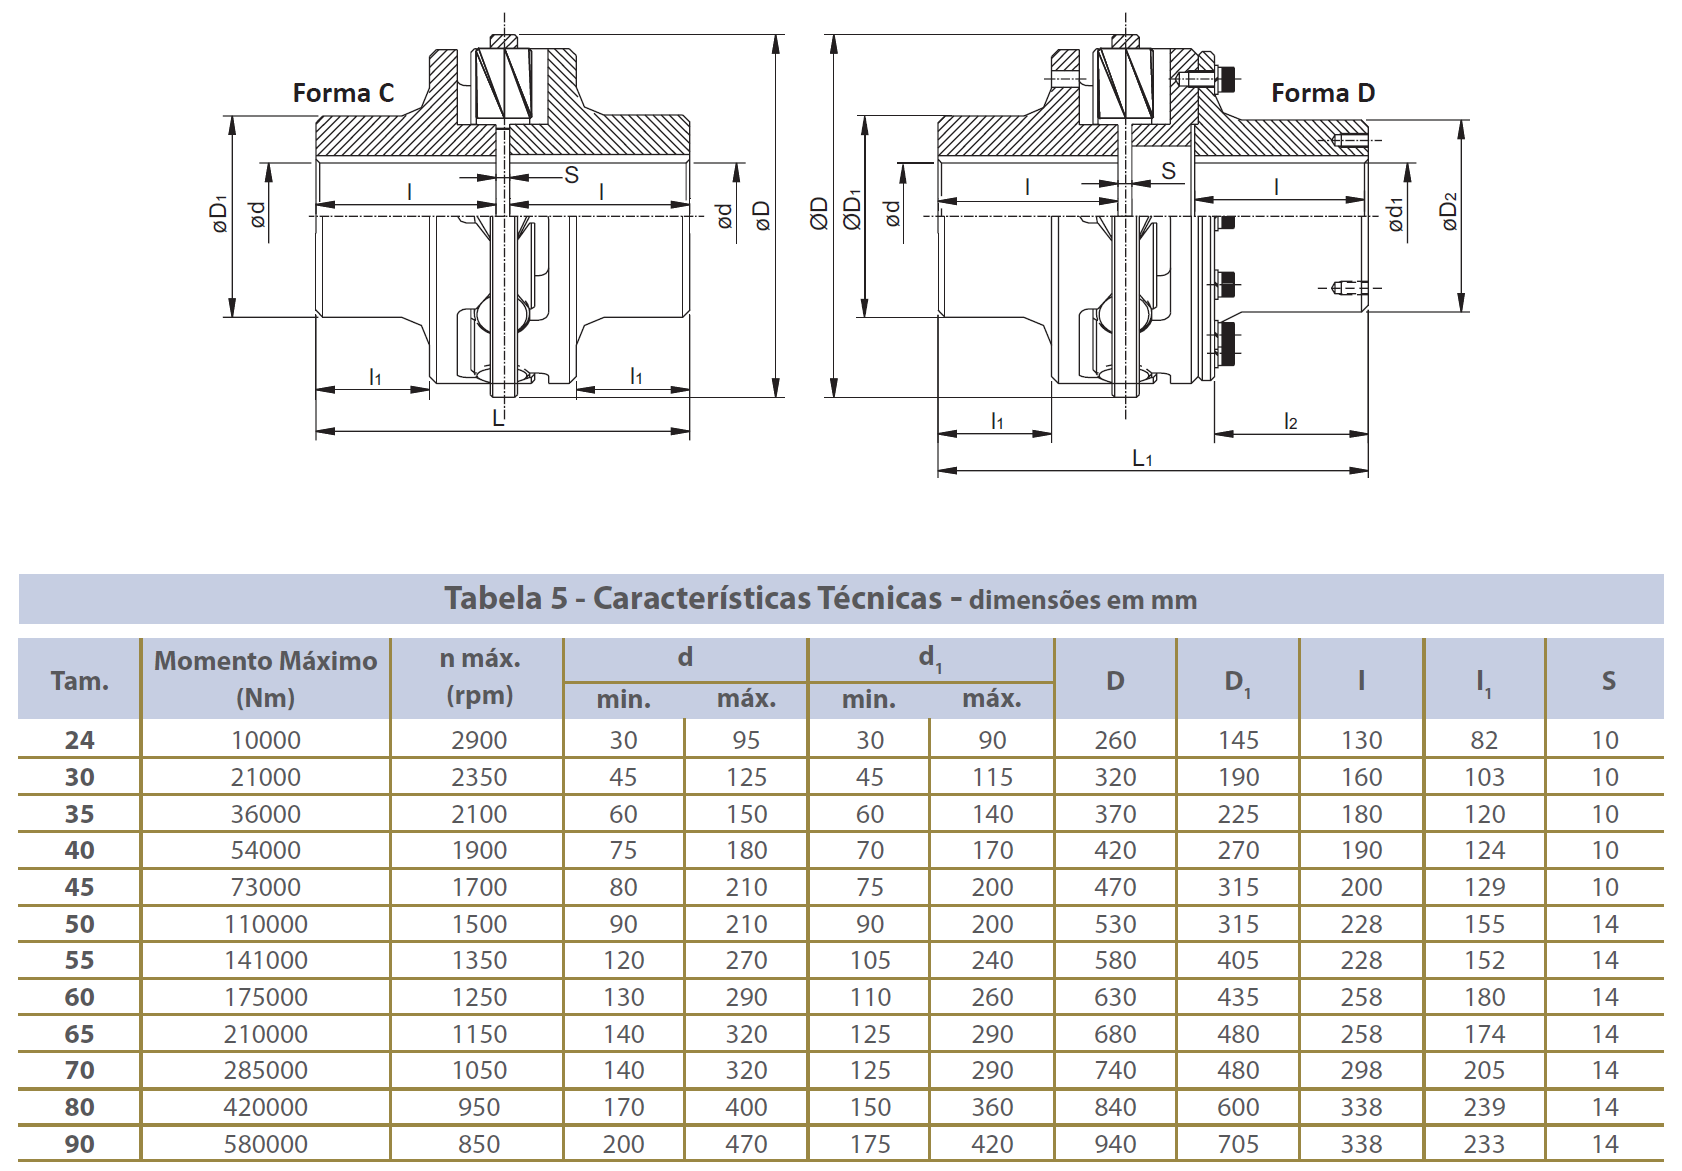
\includegraphics[width=0.7\textwidth]{content/sections/03_sistema_de_elevacao/sections/12_acoplamento_motor_redutor/images/acoplamento_motor_redutor.png}
  \caption{Catálogo de acoplamentos \cite[p.~2]{weg_cestari_acoplamentos}}
  \label{fig:acoplamento_motor_redutor}
\end{figure}

\begin{table}[H]
  \centering
  \caption{Dados do acoplamento adotado segundo o catálogo da WEG Cestari}
  \label{tab:dados_acoplamento_adotado}
  \begin{tabularx}{\textwidth}{>{\centering\arraybackslash}X>{\centering\arraybackslash}X>{\centering\arraybackslash}X}
    \toprule
    Descrição               & Símbolo                  & Valor                     \\
    \midrule
    Diâmetro mínimo do eixo & $d_{\text{min}}$         & \SI{30}{\milli\meter}     \\
    Diâmetro máximo do eixo & $d_{\text{max}}$         & \SI{95}{\milli\meter}     \\
    Rotação máxima          & $n_{\text{max}}$         & \SI{2900}{\rpm}           \\
    Torque máximo           & $T_{\text{max}}$         & \SI{10000}{\newton\meter} \\
    Massa                   & $M_{\text{acoplamento}}$ & \SI{50}{\kilo\gram}       \\
    \bottomrule
  \end{tabularx}
\end{table}
